\documentclass[12pt]{article}
\usepackage[english]{babel}
\usepackage{graphicx, amsmath, amsfonts, caption, amsthm, mathtools, listings, color, rotating, subfigure, fullpage, textcomp, setspace, enumerate, hyperref, floatrow}
\newfloatcommand{capbtabbox}{table}[][\FBwidth]

\lstset{
	language=R,
	keywordstyle=\bfseries\ttfamily\color[rgb]{0,0,1},
	identifierstyle=\ttfamily,
	commentstyle=\color[rgb]{0.133,0.545,0.133},
	stringstyle=\ttfamily\color[rgb]{0.627,0.126,0.941},
	showstringspaces=false,
	basicstyle=\tiny,
	numberstyle=\scriptsize,
	numbers=left,
	stepnumber=1,
	numbersep=10pt,
	tabsize=2,
	breaklines=true,
	breakatwhitespace=false,
	aboveskip={1.5\baselineskip},
  columns=fixed,
  upquote=true,
  extendedchars=true,
}
\title{Predicting Incidence of West Nile Virus in Chicago}
\author{Christopher Aden}
\date{\today}

\begin{document}
\maketitle

\section{Introduction}
West Nile virus (WNv) is a virus transmitted through mosquitos. If a mosquito is infected and takes a human blood-meal, there is about a 20\% chance that the individual will become infected, with symptoms including fever, neurological damage, or death. As mosquitos lay their eggs in still water and require warmer climate, WNv tends to occur most often in the summer time \cite{ruiz2009local}.

The city of Chicago experienced its first cases in 2002, and within two years, The Department of Public Health (CDPH) had established surveillance programs to track the spread of WNv, and control programs to reduce the incidence. As part of their efforts to track the virus, CDPH has released data and asked the community to predict the conditions that lead to WNv. The data comes to us in the form of mosquito traps, containing various species of mosquito, each tested for the presence of West Nile virus. The traps are mapped to a nearby address and labeled with latitude and longitude. 

Later, CDPH determines which traps had high numbers of mosquitoes and sprays an insecticide in an effort to lower the number of infected mosquitoes. This data is given as a geo-tagged set of time-stamps (latitude, longitude, date). 

Finally, Chicago has two weather stations at its airports. These stations provide valuable daily data about weather conditions, including temperature, precipitation, wind speed and direction, and so on.

Given weather, trap, and spray data, this paper will attempt to answer four central questions:
\begin{enumerate}
\item Controlling for location effects, is spraying an effective method of reducing the incidence of West Nile virus?
\item What are the main weather conditions that influence West Nile virus incidence and how do they influence it?
\item Given all data, can we accurately predict the probability that a particular mosquito species in a given trap will have West Nile virus?
\item Can we develop a statistical tool that has a useful sensitivity to detect West Nile virus, while still keeping the specificity high?
\end{enumerate}
The first two questions are inferential in nature, while the third is a prediction problem. The paper is divided accordingly, as the methods used are largely independent.

\section{Inference and Exploratory Analysis}
While predictive modeling has come into popularity in the last several years, there is still a need for inference to determine the direction and presence of significant effects. In this section, we explore how each predictor (trap, spray, and weather) affects the incidence of WNv.

We begin with an exploratory analysis of the trap data, which requires very little ``data wrangling'' to analyze. The trap data has $10,506$ rows (each row \emph{roughly} corresponds to one species in one trap on one day, though a row is split into multiple if there are more than 50 of one species of mosquito in a trap on a given day), 136 traps, accounting for $135,039$ mosquitoes, of which $14,519$ have WNv (prevalence $= 0.108\%$). There is sufficient a priori subject knowledge that all of the trap covariates are meaningful in explaining WNv, though potentially not all in conjunction. For example, mosquitoes lay their eggs in stagnant water. Traps located near stagnant water sources would thus be more likely to have more mosquitoes. The next logical jump would be to determine if the probability of WNv was related to the number of mosquitoes. A conditional plots looks at the conditional probability of WNv as a function of the number of mosquitoes. Indeed, it would appear that the probability of West Nile does go up as the number of mosquitoes increases, but decreases as the number of mosquitoes approaches the row maximum of fifty.
\begin{figure}[H] \center
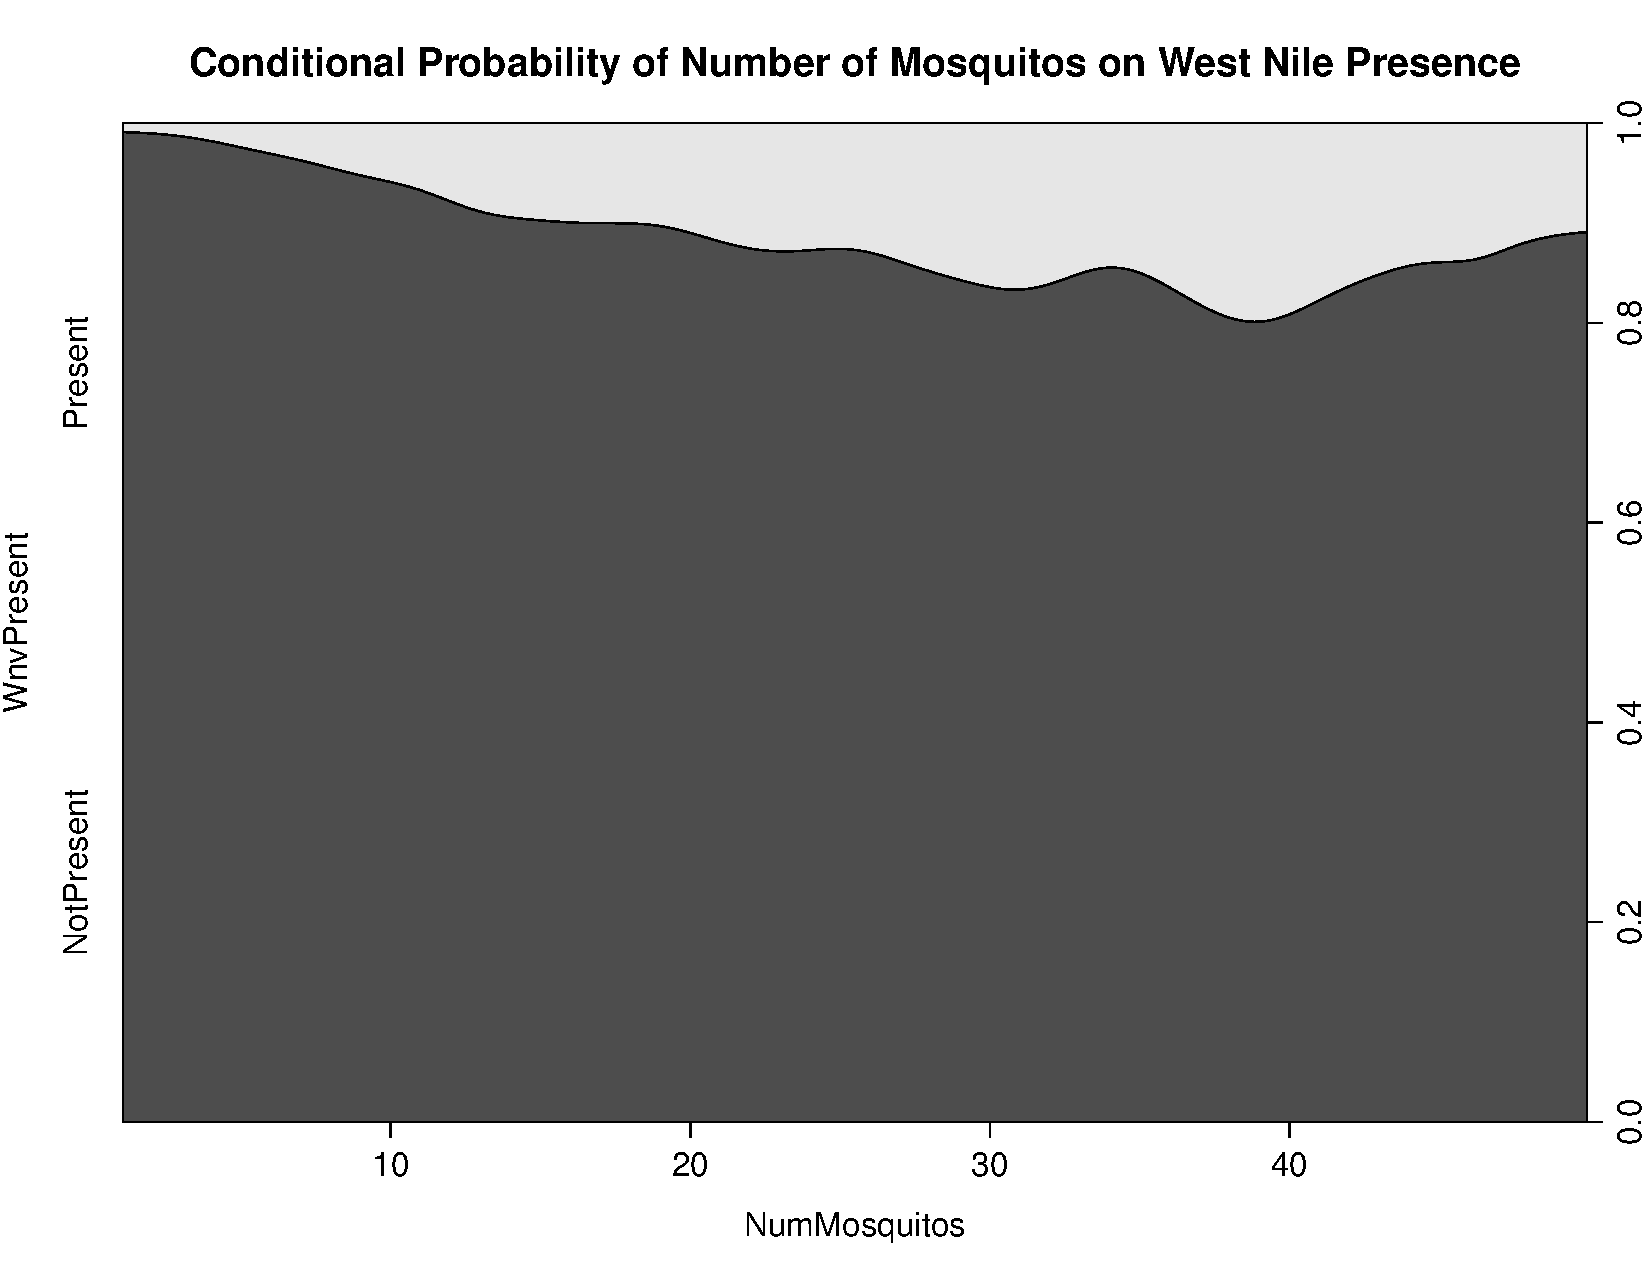
\includegraphics[scale=.30]{CD_NumMos_WNv.pdf}
\end{figure}
Do certain species of mosquito carry West Nile more frequently than others? Since our outcome (WNv present or not) and predictor (species) are categorical, mosaic plots are employed. If all species have the same incidence, the dark gray boxes, indicating WNv frequency, ought to be the same width (the height shows the species' relative frequencies). A table with the species integer mapping is provided with the mosaic plot, and it's quite clear there are differences in the prevalence.
\begin{singlespace}
\begin{figure}[H]
\begin{floatrow}
\ffigbox{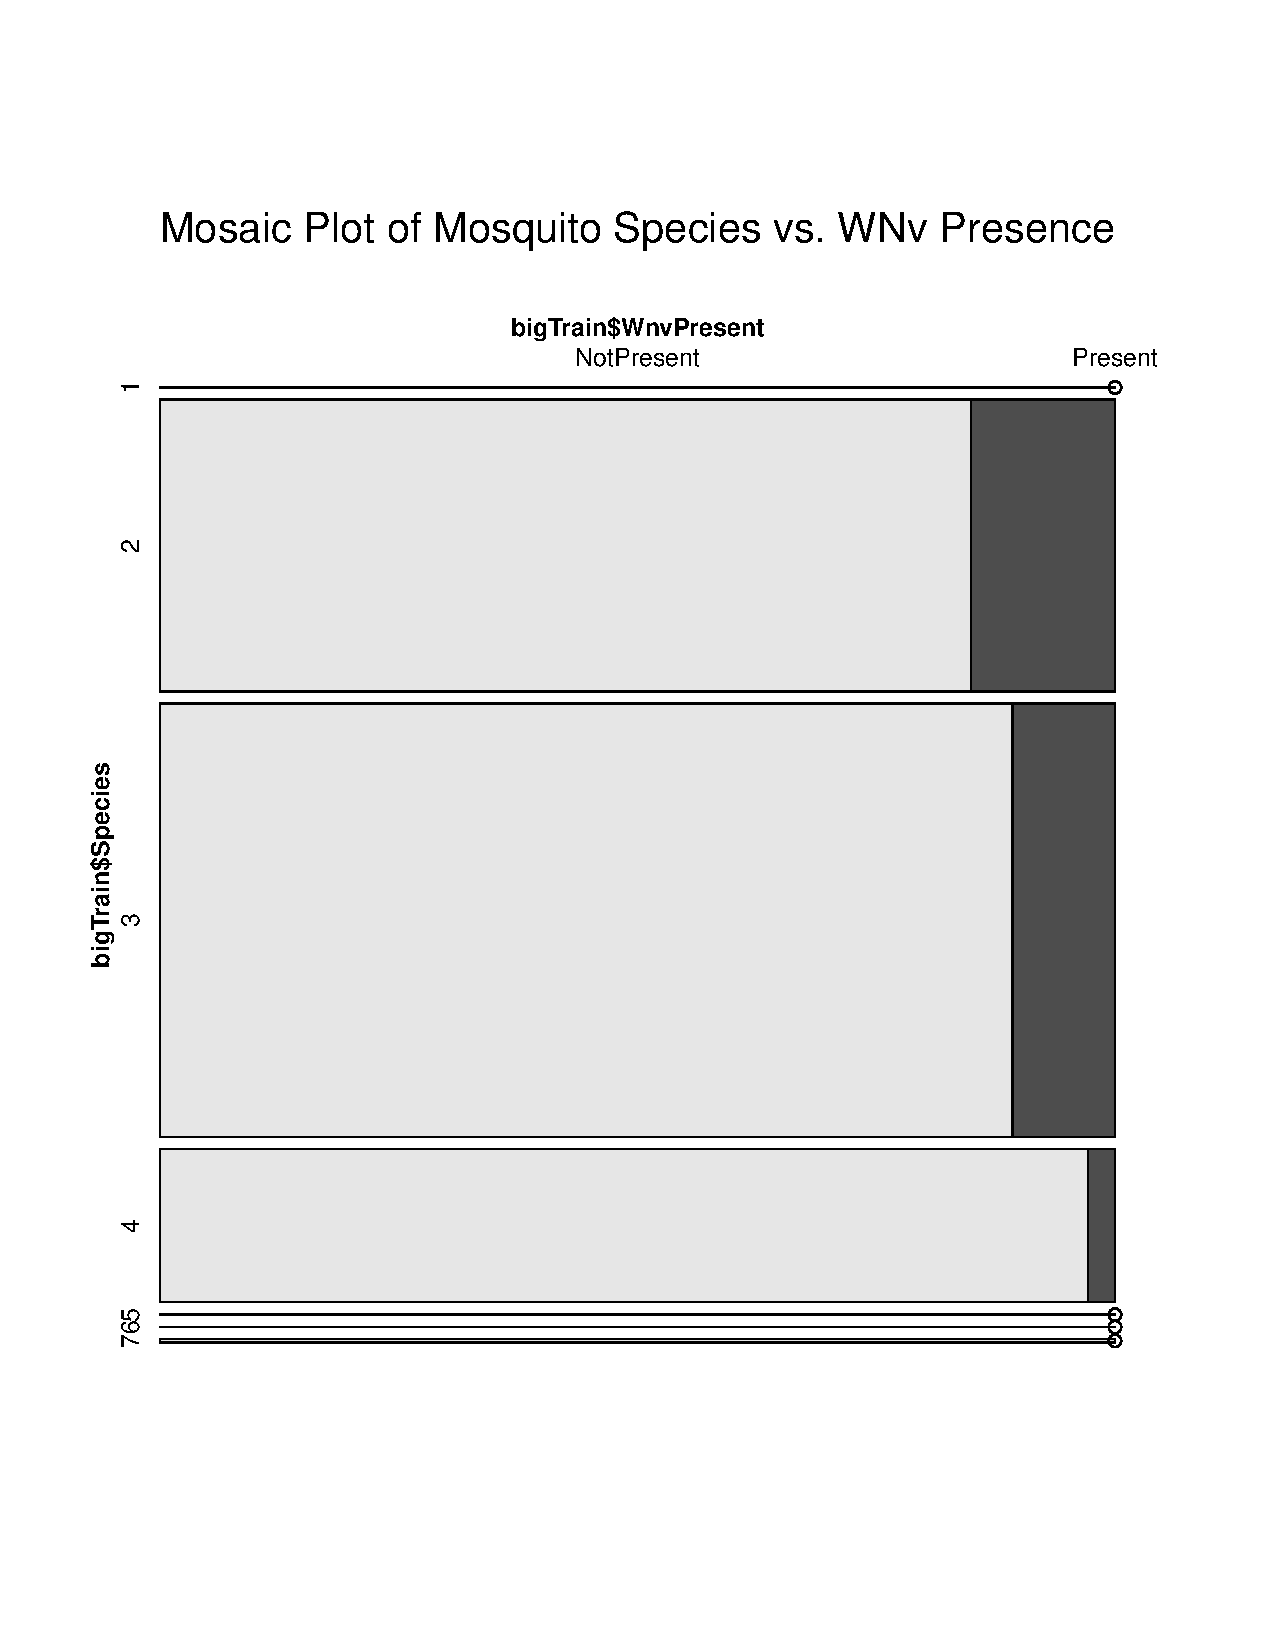
\includegraphics[height=4cm, width=8cm]{Mosaic_SpeciesVSWNv.pdf}} {\caption*{}}
\capbtabbox{
\begin{tabular}{|cc|} \hline
Key & Species \\ \hline
1 & \emph{C. Erraticus}\\ 
2 & \emph{C. Pipiens} \\ 
3 & \emph{C. Pipiens} or \emph{C. Restuans}\\ 
4 & \emph{C. Restuans} \\ 
5 & \emph{C. Salinarius} \\ 
6 & \emph{C. Tarsal} \\ 
7 & \emph{C. Territans} \\ \hline
\end{tabular}}{\caption*{}}
\end{floatrow}
\end{figure}
\end{singlespace}

In fact, the only three groups with WNv present were 2, 3, and 4, which maps to either \emph{C. Pipiens} or \emph{C. Restuans}! Previous studies confirm this result, citing \emph{C. Pipiens} \cite{turell2001vector}, \emph{C. Restuans} \cite{sardelis2001vector}, and \emph{C. Salinarius} \cite{sardelis2001vector} as confirmed vectors of WNv. As a sanity check, a Monte Carlo-based $\chi^2$ test of association between WNv presence and Species is staggeringly significant ($\chi^2 = 2472$, $p \ll .00001$), with the $p$-value limited by the number of MC simulations, indicating a likely relationship between species and WNv incidence.

Similarly, location may play a role. As we expect, conditional plots reveal that there is a clear effect of  latitude and longitude, but not a clear linear pattern on either. 
\begin{figure}[H] \center
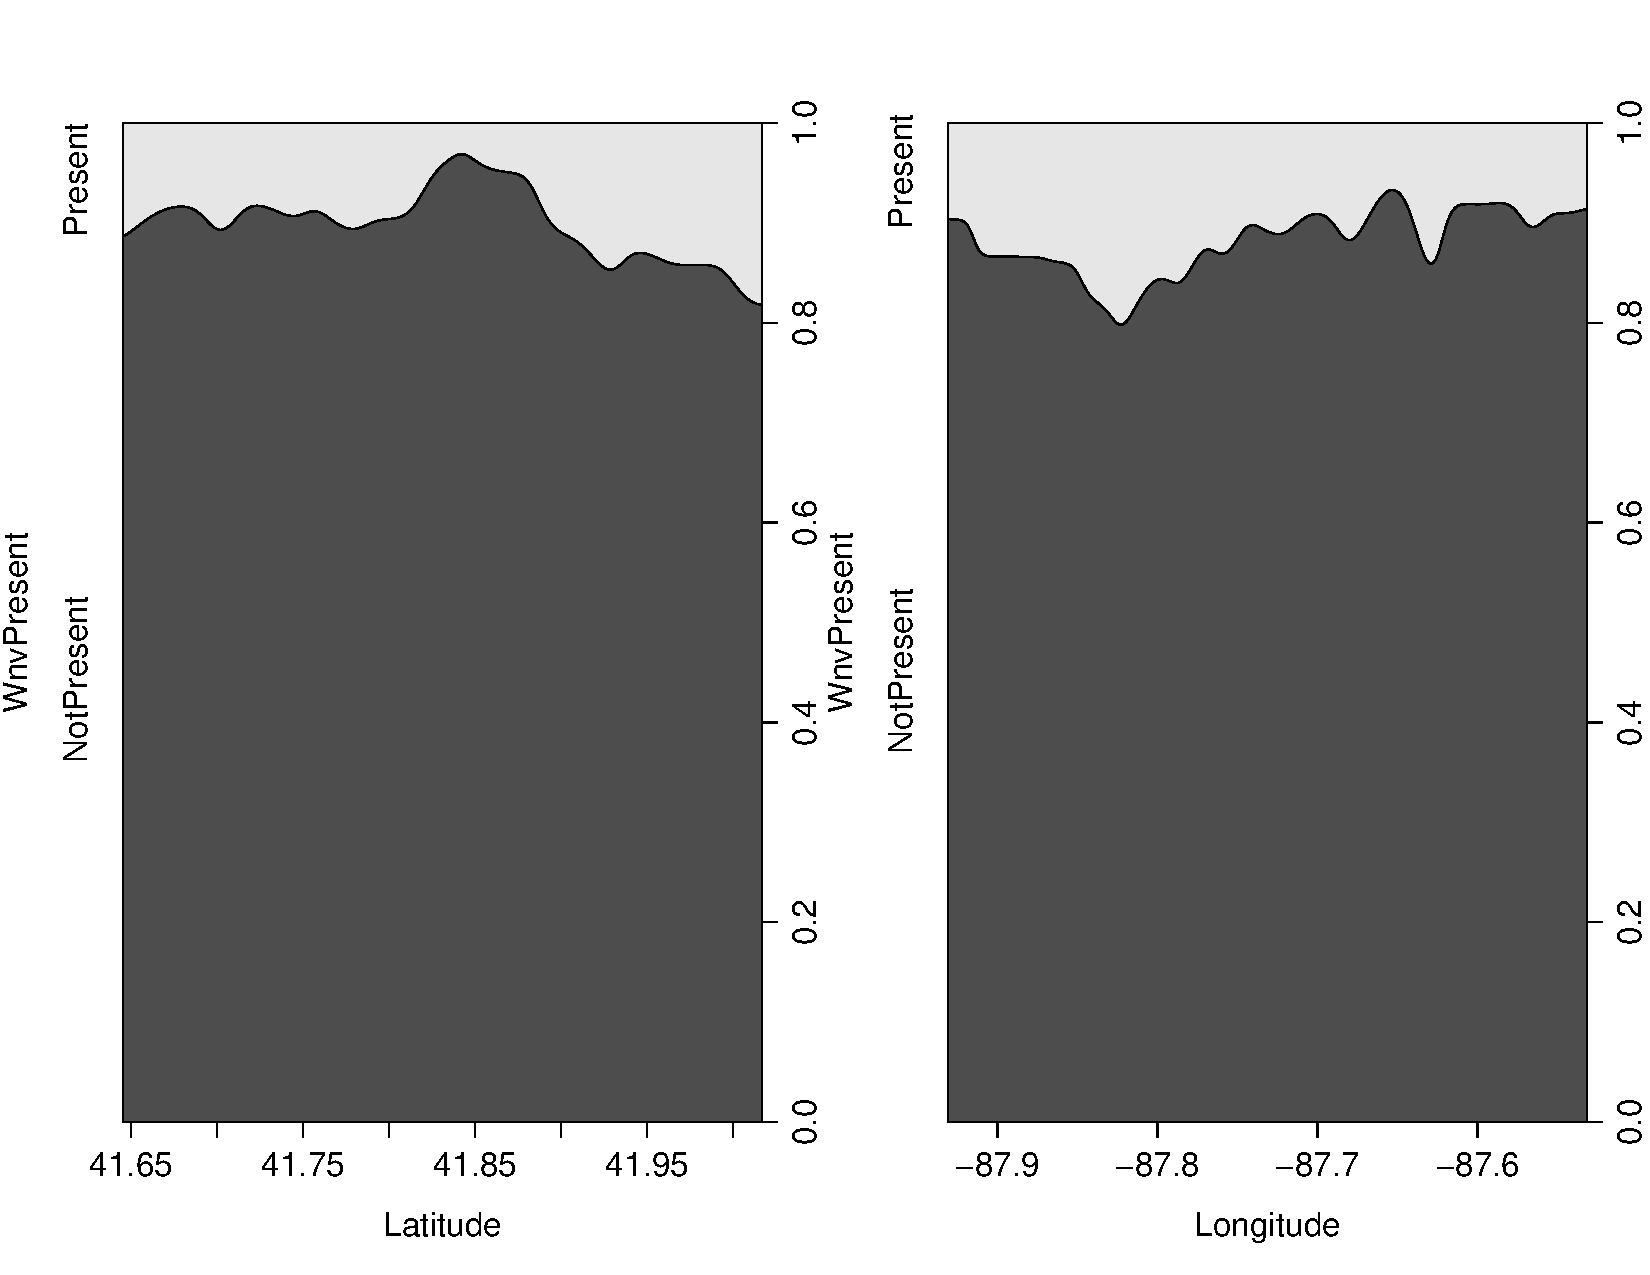
\includegraphics[scale=.30]{CD_LatLong.pdf}
\caption*{Latitude and Longitude Conditional Density Plots}
\end{figure}

We move on to spray data. This was quite a controversial piece in the Kaggle competition. Spraying data is provided only for years that are not in the set of data being judged in the competition (2011, 2013). The Inference chapter focuses only on this subset of the data that includes the spray data, while the prediction chapter will focus on both. As the administrator of the competition wrote in a reply about the insecticide spray data for the years in the testing set, ``as far as we know, they haven't been super effective in controlling the spread of WNV'' \cite{SprayQuote1} and having the sprays be tied to the prevalence of previous weeks West Nile surveillance, the inclusion of spray data ``could lead to data leakage, therefore, spray data in the test years are not provided'' \cite{SprayQuote2}. The data proved \emph{exceptionally} difficult to manage. Each spray is tagged with a latitude, longitude, and time stamp. It is plausible to believe that sprays closer in spatial and temporal proximity to a given trap (on a particular day) are more effective than sprays that happened in the previous year, or on the opposite side of town. The sophisticated way for dealing with this would be to apply a temporal-spatial model that allows for a correlation between space and time that decays exponentially (or polynomially). This is computationally and theoretically beyond the scope of this analysis. As a cheap proxy, we assume that the effective radius of a given spray is no more than two miles (the speculated range of a given mosquito), and that the spray effect has completely diminished after two weeks. This approach then counts how many sprays have occurred in the last two weeks in a two mile radius, which is \emph{still} computationally difficult, given that there are $14,294$ sprays! We pare down the size of the problem by subsetting our trap data to only the years we have spray data for, which gives $4,446$ latitude-longitude pairs. Euclidean distance is an extremely poor metric for map distances, because the Earth is not a flat surface. Relative errors for using Euclidean geometry can be quite high. To overcome this, we use the Haversine formula, designed especially for computing distances on spheres. For two latitude-longitude pairs $(\phi_1, \lambda_1)$, $(\phi_2, \lambda_2)$, the Haversine Formula gives $d$ as
\[ d = 2 r \arcsin\left(\sqrt{\sin^2\left(\frac{\phi_2 - \phi_1}{2}\right) + \cos(\phi_1) \cos(\phi_2)\sin^2\left(\frac{\lambda_2 - \lambda_1}{2}\right)}\right), \]
where $r$ is the radius of the Earth ($3,959$ mi). We then compute all $(14,294)(4,446) = 63,551,124$ distances and determine which are less than two miles, then filter only the recently-occurring sprays. The result is reduced one more time to give an integer of the number of spatiotemporally-proximal sprays for each trap-day.

The vast majority of traps have not experienced a recent spray ($.946\%$). Histograms of nearby sprays with and without the zero sprays are included in subsection two of the Appendix. This is important for analysis when we look at the conditional density plots. We won't see a change in the conditional density until the $95^{th}$ percentile of sprays, distorting the picture. Excluding the zeroes, there is a clear difference in the density over sprays, but not in any clear way.
\begin{figure}[H] \center
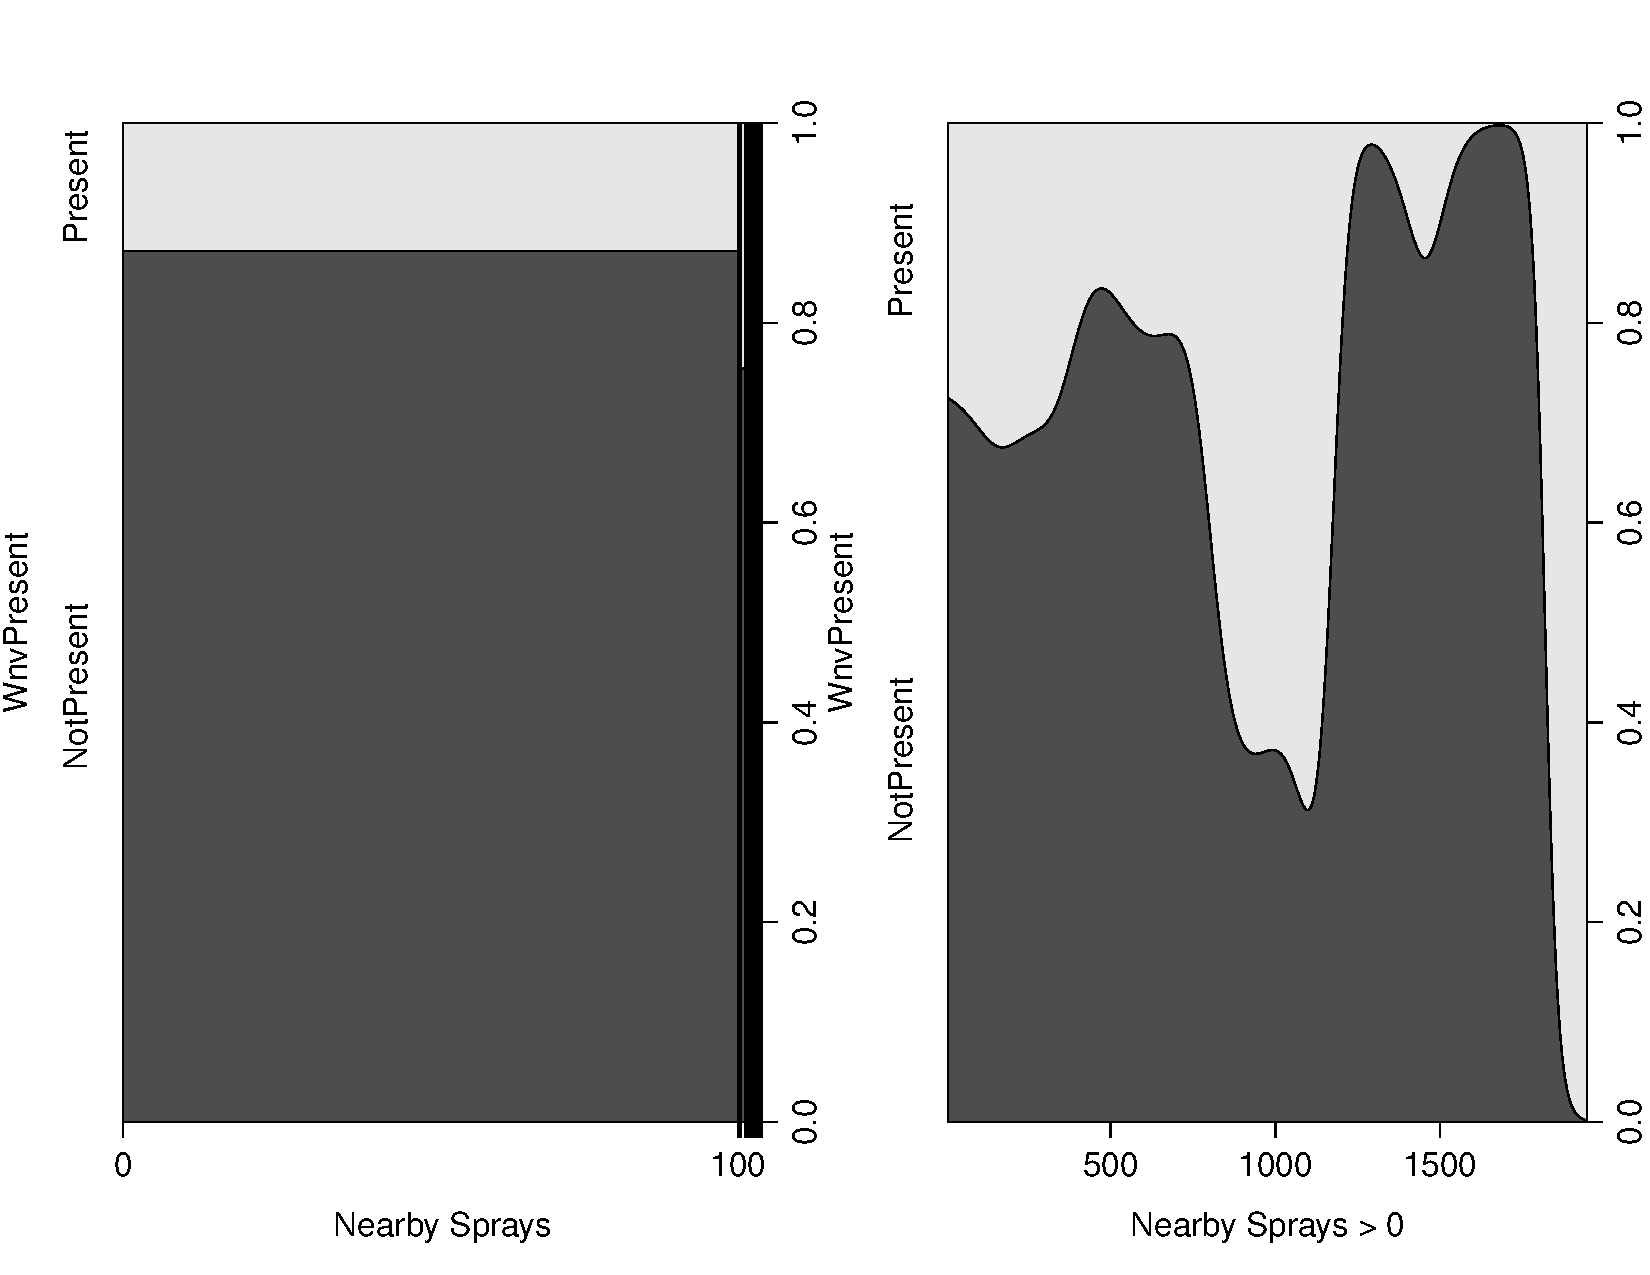
\includegraphics[scale=.35]{CD_NearbySpraysVSwnv.pdf}
\caption*{Zero included (left) and excluded (right) Proximal Spray Count Conditional Densities}
\end{figure}

Weather data is much simpler. Each of the two weather stations (located at O'Hare International Airport and Midway International Airport) recorded weather data every day over the course of the study. We continue to focus only on the data we have sprays for (years 2011 and 2013, $n=55,243$). We begin by averaging the two weather stations' observations together (the differences between the two stations is relatively small), then merging the weather data to the trap data through the date on each weather record. Collected weather data and descriptions are available through NOAA's Quality Controlled Local Climatological Data documentation (\url{http://www.ncdc.noaa.gov/qclcd/qclcddocumentation.pdf}). We will skip description of the exploratory analysis on the weather data. Prior work\cite{ruiz2009local} suggests that air temperature and low humidity play very significant roles in human infection rates of West Nile virus, and potentially other factors could play significant roles, too. Logistic regression models that incorporate all variables mentioned in the NOAA QCLCD documentation, our spray data, and our trap data are included in the appendix. One model includes proximal sprays as a continuous term, while the other dichotomizes it to whether it is nonzero or not. However, both models lack parsimony. Additionally, it is very likely that the predictors are highly correlated, due to our inclusion of an interaction term for longitude and latitude of the trap. The interaction allows the odds of WNv to increase not just North-South or East-West, but in more complicated directions. 

At this point, we pursue model selection, which requires caution. To avoid over-fitting (reporting a model that is more significant than in reality by training the model on the same data as the test set), we train on 80\% of the observations and withhold 20\% to test the model's validity. We perform ridge regression on the dichotomized model to reduce the collinearity, but this proves somewhat futile. Ridge regression performs very admirably at reducing the variance inflation factors (see table in Appendix), but the model still has unacceptably large collinearity. What we really need is to drop terms entirely from the model. This is where we employ ElasticNet \cite{zou2005regularization}, a hybrid penalization method that minimizes
\[ \frac{1}{N} \sum_{i=1}^{N} w_i l(y_i,\beta_0+\beta^T x_i) + \lambda\left[(1-\alpha)||\beta||_2^2/2 + \alpha ||\beta||_1\right], \]
where $\alpha$ determines the balance between ridge regression and lasso, and $\lambda$ is the tuning parameter. ElasticNet is a combination of L2 (ridge regression) and L1 (lasso) penalties, allowing terms to drop from the model completely, while avoiding lasso's drawback of keeping only one similar predictor in the final model. \verb+R+'s implementation, \verb+glmnet+, optimizes $\lambda$ for a fixed $\alpha$. Commonly, $\alpha$ is kept close to either 0 (for ridge) or 1 (for lasso). We leave it as .9 to mimic lasso to get a simplistic model. Using cross-validation, we find the $\lambda$ that minimizes the deviance, then run lasso with a $\lambda$ that is one standard deviation larger for increased parsimony. The terms of the model reduced to zero are dropped, and the reduced model is tested on the withheld data ($n=11,049$).

This model is far easier to read and terms are significant even in the testing data. Some terms are not statistically significant, but the testing data set is also \emph{much} smaller than the training set. The variance inflation factors have largely stabilized, except for StationPressure and SeaLevel, which measure the air pressure at the weather station and sea level, respectively, so collinearity is to be expected. Removing the sea level pressure makes the station pressure extremely significant, and the VIFs stabilize. In the face of the ElasticNet's recommendation, it may be prudent to keep only the weather station pressure.

\begin{footnotesize}
\begin{tabular}{|c|cccc|} \hline
& Estimate & SE & $z$-value & $p$-value \\ \hline
(Intercept) & -470.5712 & 44.66 & -10.54 & $\ll 0.0001$ \\ 
isSpecies1247TRUE & -0.1289 & 0.06 & -2.05 & 0.0405 \\ 
Longitude & -3.7336 & 0.60 & -6.21 & $\ll 0.0001$ \\ 
Year2013 & 0.6037 & 0.11 & 5.70 & $\ll 0.0001$ \\ 
Month7 & 2.3112 & 0.42 & 5.51 & $\ll 0.0001$ \\ 
Month8 & 4.6864 & 0.42 & 11.28 & $\ll 0.0001$ \\ 
Month9 & 4.4322 & 0.42 & 10.66 & $\ll 0.0001$ \\ 
Tmax & 0.0712 & 0.01 & 8.34 & $\ll 0.0001$ \\ 
HeatDegreeDay & 0.0781 & 0.02 & 3.19 & 0.0014 \\ 
StationPressure & 3.9241 & 0.70 & 5.60 & $\ll 0.0001$ \\ 
ResultSpeed & 0.0980 & 0.02 & 5.74 & $\ll 0.0001$ \\ 
anyNearbySpraysTRUE & 0.5445 & 0.11 & 5.06 & $\ll 0.0001$ \\ 
Latitude:Longitude & -0.0042 & 0.005 & -0.87 & 0.3859 \\ \hline
\end{tabular} \qquad
\begin{tabular}{|cc|} \hline 
Term & VIF \\ \hline
isSpecies1247 & 1.04 \\ 
Longitude & 4.08 \\ 
Year & 1.89 \\ 
Month & 2.07 \\ 
Tmax & 3.97 \\ 
HeatDegreeDay & 2.95 \\ 
StationPressure & 4.79 \\ 
ResultSpeed & 2.98 \\ 
anyNearbySprays & 1.08 \\ 
Latitude:Longitude & 4.04 \\ \hline
\end{tabular}
\end{footnotesize}

We can also try a generalized additive model with a tensor product interaction term. Looking at conditional density plots gives us an idea which terms are highly nonlinear. It turns out nearly all of them, though HeatDay is poorly-behaved. Output from the GAM approach is attached in the appendix. This approach is far superior at modeling the latitude and longitude, as the linearity assumption in the logistic regression is too strict for something like a location, but it lacks the interpretability of logistic regression. The additional terms also mean we lose power--nearly all coefficients are now not significant, except for the spray effect and location effect. A less nuclear approach would be to only make smooth terms for the location and leave everything else as linear, despite their nonlinearity. While this would not capture the nuances of their relationships, we would not take such a large penalty to our degrees of freedom.

Finally, it is quite likely that within a specific trap, there will be correlations. This is due not only due to similar location, but that mosquitoes in the same trap may have behaved similarly in contracting WNv themselves. We attempt to model this with a random effect for the specific trap. Since our goal is to make a statement about the average trap, the marginal random effects model is most appropriate. We choose an exchangeable correlation structure (all mosquitoes within a trap share one common correlation) for computational feasibility, though at this sample size, sandwich estimators asymptotics are valid, and our choice of correlation structure is less important. Output is attached in the appendix, and shows a strong effects from longitude, year, month, and proximity to an insecticide spray. Species and weather conditions were not significant in this model.

\section{Prediction}
Statistical inference has its place in the planning room, determining which predictors are most meaningful in explaining the odds of WNv, but prediction problems has its place in the field. While we produced a model and analyzed the predictors that most impacted incidence of West Nile virus, generalized linear models are rarely the best tools if the only goal is prediction, as they are forced to obey the rigid linearity constraint (through the linear predictor). In this section, we disregard any notion of statistical significance and instead strive to achieve a high rate of predictive accuracy. The realistic motivation for this section is that once we have collected weather and trap data, we want the most accurate possible prediction for whether a given mosquito has West Nile virus.

There are two main aims for this section. First, we will create models that try to predict WNv as accurately as possible. Second, we will evaluate metrics subjectively, assessing whether they meet our needs for sensitivity and specificity jointly. 

As a comparison of the more modern machine learning methods used in the section, each subset and each metric will be compared against a logistic regression and ElasticNet model. The simplicity of both approaches lends itself well to interpretability, and it may be useful to use them for prediction. The primary computational tool employed is the \verb+R+ package \verb+caret+, which has a parallel grid-search optimizer for algorithm parameters and has cross-validation and output methods built-in. In each case, metrics are estimated using 5-fold cross-validation, training on 80\% of the data, then estimating the metric with the remaining 20\%. 
A short description of each predictive model used is as follows:
\begin{enumerate}
\item Logistic Regression: A full logistic regression, with no model selection.
\item ElasticNet Logistic Regression: A full logistic regression followed by a grid-search for optimal $(\alpha, \lambda)$ to use in an ElasticNet.
\item RandomForest\cite{breiman2001random}: A tree-based ensemble method where a combination of trees, each one taking a random subset of the data \emph{and} a random subset of the \emph{predictors}, are averaged to create a consensus classifier.
\item Adaptive Boosting (AdaBoost) \cite{Schapire99improvedboosting}: An ensemble method that combines the information from trees that show very little improvement over guessing (like a decision tree with only one split), then tunes subsequent trees to perform better on the samples that the previous trees misclassified.
\item Gradient Boosting Machines\cite{friedman2001greedy}: A more general class of ensemble methods that includes AdaBoost. GBMs allow for more general (differentiable) loss functions, and optimizes using gradient descent with a modification to control the rate of descent.
\end{enumerate}

Since the aim of the section is to optimize our classification rate, we will look at three different subsets of the data:
\begin{enumerate}
\item Use the trap and weather data from all available years (2007, 2009, 2011, 2013).
\item Use the trap, weather, and spray data from years in which we have insecticide spray data (2011, 2013) and see how well on held-out data from the same years (as a way to judge how effective spray data is as for classification).
\item Use trap and weather data from just the years we have spray data. The goal is to answer how much worse model quality would be without spray data.
\end{enumerate}

This model-free approach would usually be quite problematic, due to concerns of overfitting and data-snooping, but we solve this problem by snooping on the training set and validating on the test set. The ensemble methods also do their own built-in withholding of data, either by operating on weak learners, or using only a subset of the data at a time. These more advanced machine learning techniques are never given a full glimpse of the data at any one time. As a naive criterion, we might seek to maximize the AUC or minimize the misclassification rate (sum of the false negative and false positive rates). A 5-fold cross-validated confusion matrix shows us the proportional breakdown of negatives and positives for each method.

\begin{table}[H] \center \footnotesize
\begin{tabular}{|ll|rrrr|} \hline
Method & Data & True Neg & False Neg & False Pos & True Pos \\ \hline
GLM & AllYears, Weather & 89.10 & 10.50 & 0.10 & 0.30 \\ 
  ElasticNet & AllYears, Weather & 89.10 & 10.60 & 0.10 & 0.10 \\ 
  RandomForest & AllYears, Weather & 88.30 & 4.00 & 0.90 & 6.70 \\ 
  GradientBoosting & AllYears, Weather & 87.80 & 6.20 & 1.50 & 4.60 \\ 
  AdaBoost & AllYears, Weather & 88.40 & 9.20 & 0.80 & 1.60 \\ \hline
  GLM & SprayYears, Weather & 86.10 & 12.50 & 0.50 & 0.90 \\ 
  ElasticNet & SprayYears, Weather & 86.20 & 12.70 & 0.40 & 0.70 \\ 
  RandomForest & SprayYears, Weather & 85.00 & 3.20 & 1.60 & 10.20 \\ 
  GradientBoosting & SprayYears, Weather & 84.40 & 5.00 & 2.20 & 8.40 \\ 
  AdaBoost & SprayYears, Weather & 84.60 & 8.80 & 2.00 & 4.60 \\ \hline
  GLM & SprayYears, SprayWeather & 86.10 & 12.40 & 0.50 & 1.00 \\ 
  ElasticNet & SprayYears, SprayWeather & 86.10 & 12.50 & 0.50 & 0.90 \\ 
  RandomForest & SprayYears, SprayWeather & 85.10 & 3.30 & 1.50 & 10.10 \\ 
  GradientBoosting & SprayYears, SprayWeather & 84.50 & 5.00 & 2.10 & 8.40 \\ 
  AdaBoost & SprayYears, SprayWeather & 84.50 & 9.00 & 2.10 & 4.40 \\ \hline
\end{tabular}
\end{table}

The models all achieve remarkable accuracy, but they do so by predicting no WNv almost every time! This is a well-studied problem with prediction problems. The problem is that the metric is a poor choice to optimize when the classes (presence and non-presence of WNv) are not close to 50-50. Realistically, we are willing to take a hit in overall accuracy (losing specificity) if it means gaining much more sensitivity. This is because a model that cannot predict a positive when a mosquito actually has WNv has no predictive power. The problem is solved by instead choosing one of two different metrics that attempts to punish classifiers that try to ``cheat'' and use the unbalanced classes to their advantage.

\begin{enumerate}
\item $F_1$ Score\cite{powers2011evaluation}: $F_1 = 2 \cdot \left( \mathrm{PPV} \cdot \mathrm{Sens} \right) / \left( \mathrm{PPV} + \mathrm{Sens}\right)$, is a metric that strives to have a high sensitivity (probability of predicting WNv when a mosquito actually has WNv), but weights it according to the positive predictive value (probability of a mosquito having WNv when I have predicted it to be present). With the GLM model using only weather data on all years, for example, $F_1$ would be $F_1 = 2 \cdot ( (.03/.04) \cdot (0.3 / 10.8)) / ( (.03/.04) + (0.3 / 10.8)) = 0.054$. Predicting all mosquitoes as WNv-free would give an $F_1$ score of $0$, so the classifier is not fairing well.

\item Balanced Accuracy\cite{brodersen2010balanced}: The easier to understand of the two metrics, balanced accuracy is the mean of the specificity and sensitivity. In the accuracy-optimizing case, the models perform well by achieving a high specificity and sacrificing their sensitivity. With balanced accuracy, this cannot be done without taking a large penalty. With the GLM model using only weather data on all years, for example, balanced accuracy would be $BA = ((89.1/89.2) + (0.3 / 10.8)) / 2 = 0.513$. Predicting everyone to belong to one class results in a balanced accuracy of $.50$, so this metric does indeed correct the greediness of optimizing for total accuracy.
\end{enumerate}

Re-running these models, optimizing now for $F_1$ and $BA$, we come up with much more realistic confusion matrices. 
\begin{table}[H] \center \footnotesize
\begin{tabular}{|ll|rrrrr|} \hline
Method & Data & True Neg & False Neg & False Pos & True Pos & F1 \\ \hline
GLM & AllYears, Weather & 89.10 & 10.50 & 0.10 & 0.30 & 0.05 \\ 
  ElasticNet & AllYears, Weather & 89.10 & 10.50 & 0.10 & 0.20 & 0.04 \\ 
  RandomForest & AllYears, Weather & 88.30 & 4.00 & 1.00 & 6.80 & 0.73 \\ 
  GradientBoosting & AllYears, Weather & 87.90 & 6.30 & 1.40 & 4.50 & 0.54 \\ 
  AdaBoost & AllYears, Weather & 88.40 & 9.10 & 0.80 & 1.70 & 0.26 \\ 
  GLM & SprayYears, Weather & 86.10 & 12.50 & 0.50 & 0.90 & 0.12 \\ 
  ElasticNet & SprayYears, Weather & 86.50 & 12.90 & 0.00 & 0.50 & 0.07 \\ 
  RandomForest & SprayYears, Weather & 85.20 & 3.40 & 1.40 & 10.00 & 0.81 \\ 
  GradientBoosting & SprayYears, Weather & 85.30 & 10.50 & 1.30 & 2.90 & 0.33 \\ 
  AdaBoost & SprayYears, Weather & 84.60 & 8.80 & 2.00 & 4.70 & 0.47 \\ 
  GLM & SprayYears, SprayWeather & 86.10 & 12.40 & 0.50 & 1.00 & 0.13 \\ 
  ElasticNet & SprayYears, SprayWeather & 86.40 & 12.80 & 0.20 & 0.60 & 0.09 \\ 
  RandomForest & SprayYears, SprayWeather & 85.10 & 3.30 & 1.50 & 10.10 & 0.81 \\ 
  GradientBoosting & SprayYears, SprayWeather & 85.40 & 10.20 & 1.20 & 3.20 & 0.36 \\ 
  AdaBoost & SprayYears, SprayWeather & 84.50 & 8.70 & 2.10 & 4.70 & 0.47 \\ \hline
\end{tabular}
\caption*{Confusion Matrices for $F_1$-based optimization}
\end{table}

\begin{table}[H] \center \footnotesize
\begin{tabular}{|ll|rrrrr|} \hline
Method & Data & True Neg & False Neg & False Pos & True Pos & BA \\ \hline
GLM & AllYears, Weather & 89.10 & 10.50 & 0.10 & 0.30 & 0.51 \\ 
  ElasticNet & AllYears, Weather & 89.10 & 10.50 & 0.10 & 0.20 & 0.51 \\ 
  RandomForest & AllYears, Weather & 88.20 & 3.90 & 1.00 & 6.80 & 0.81 \\ 
  GradientBoosting & AllYears, Weather & 87.80 & 6.60 & 1.50 & 4.10 & 0.68 \\ 
  AdaBoost & AllYears, Weather & 88.40 & 9.10 & 0.80 & 1.60 & 0.57 \\ 
  GLM & SprayYears, Weather & 86.10 & 12.50 & 0.50 & 0.90 & 0.53 \\ 
  ElasticNet & SprayYears, Weather & 86.00 & 12.50 & 0.50 & 0.90 & 0.53 \\ 
  RandomForest & SprayYears, Weather & 85.00 & 3.20 & 1.50 & 10.20 & 0.87 \\ 
  GradientBoosting & SprayYears, Weather & 84.50 & 5.20 & 2.10 & 8.30 & 0.80 \\ 
  AdaBoost & SprayYears, Weather & 84.60 & 8.80 & 2.00 & 4.60 & 0.66 \\ 
  GLM & SprayYears, SprayWeather & 86.10 & 12.40 & 0.50 & 1.00 & 0.53 \\ 
  ElasticNet & SprayYears, SprayWeather & 86.10 & 12.50 & 0.50 & 0.90 & 0.53 \\ 
  RandomForest & SprayYears, SprayWeather & 84.90 & 3.20 & 1.70 & 10.20 & 0.87 \\ 
  GradientBoosting & SprayYears, SprayWeather & 84.50 & 5.00 & 2.10 & 8.40 & 0.80 \\ 
  AdaBoost & SprayYears, SprayWeather & 84.50 & 9.00 & 2.10 & 4.40 & 0.65 \\ 
   \hline
\end{tabular}
\caption*{Confusion Matrices for $BA$-based optimization}
\end{table}

No one method particularly out-performs the rest, but GLMs and ElasticNets lag behind. The more sophisticated models took a hit in overall accuracy with these two metrics, but made up for it in improved positive-sample classification. In the end, that was what we cared about all along. Fitted to their respective three problems without cross-validation (to be used in the Kaggle competition), the ROC curves for the three data scenarios were created, and are attached in the Appendix. 

\section{Conclusion}
On the subject of inference, regularization allowed us to separate the wheat from the chaff, finding a very significant model, that was parsimonious and intuitive to explain. Previous weather findings from other scientists were reinforced as our model demonstrated that hot and arid conditions are most amenable to West Nile virus. There was a clear location effect, and future work would need to cover a spatial analysis, but smooth with GAM was still able to find a meaningful relationship between location and the presence of WNv.

On the topic of the competition administrator's initial comments about the number of proximal sprays not being effective at controlling the spread, the evidence is inconclusive without more sophisticated tools. The logistic model demonstrates that the sprays are at least being aimed in the right places, as there is an increased odds of WNv in places that are being sprayed, but this cannot speak to the effectiveness of the insecticide.

On the subject of prediction, high AUC's were explained by uneven frequencies. More realistic tools like $F_1$ and Balanced Accuracy were still able to salvage insight from the data, and produced very high scores, nonetheless. These models have the advantage of high sensitivity, which the accuracy-optimized models did not. Future work would focus on the spatiotemporal aspect of the data and attempt to draw conclusions about the spread of WNv over time using more advanced methods than GLMs and GLMMs.

\newpage
\section{Appendix}
\subsection{Figures and Tables}
\begin{figure}[H] \center
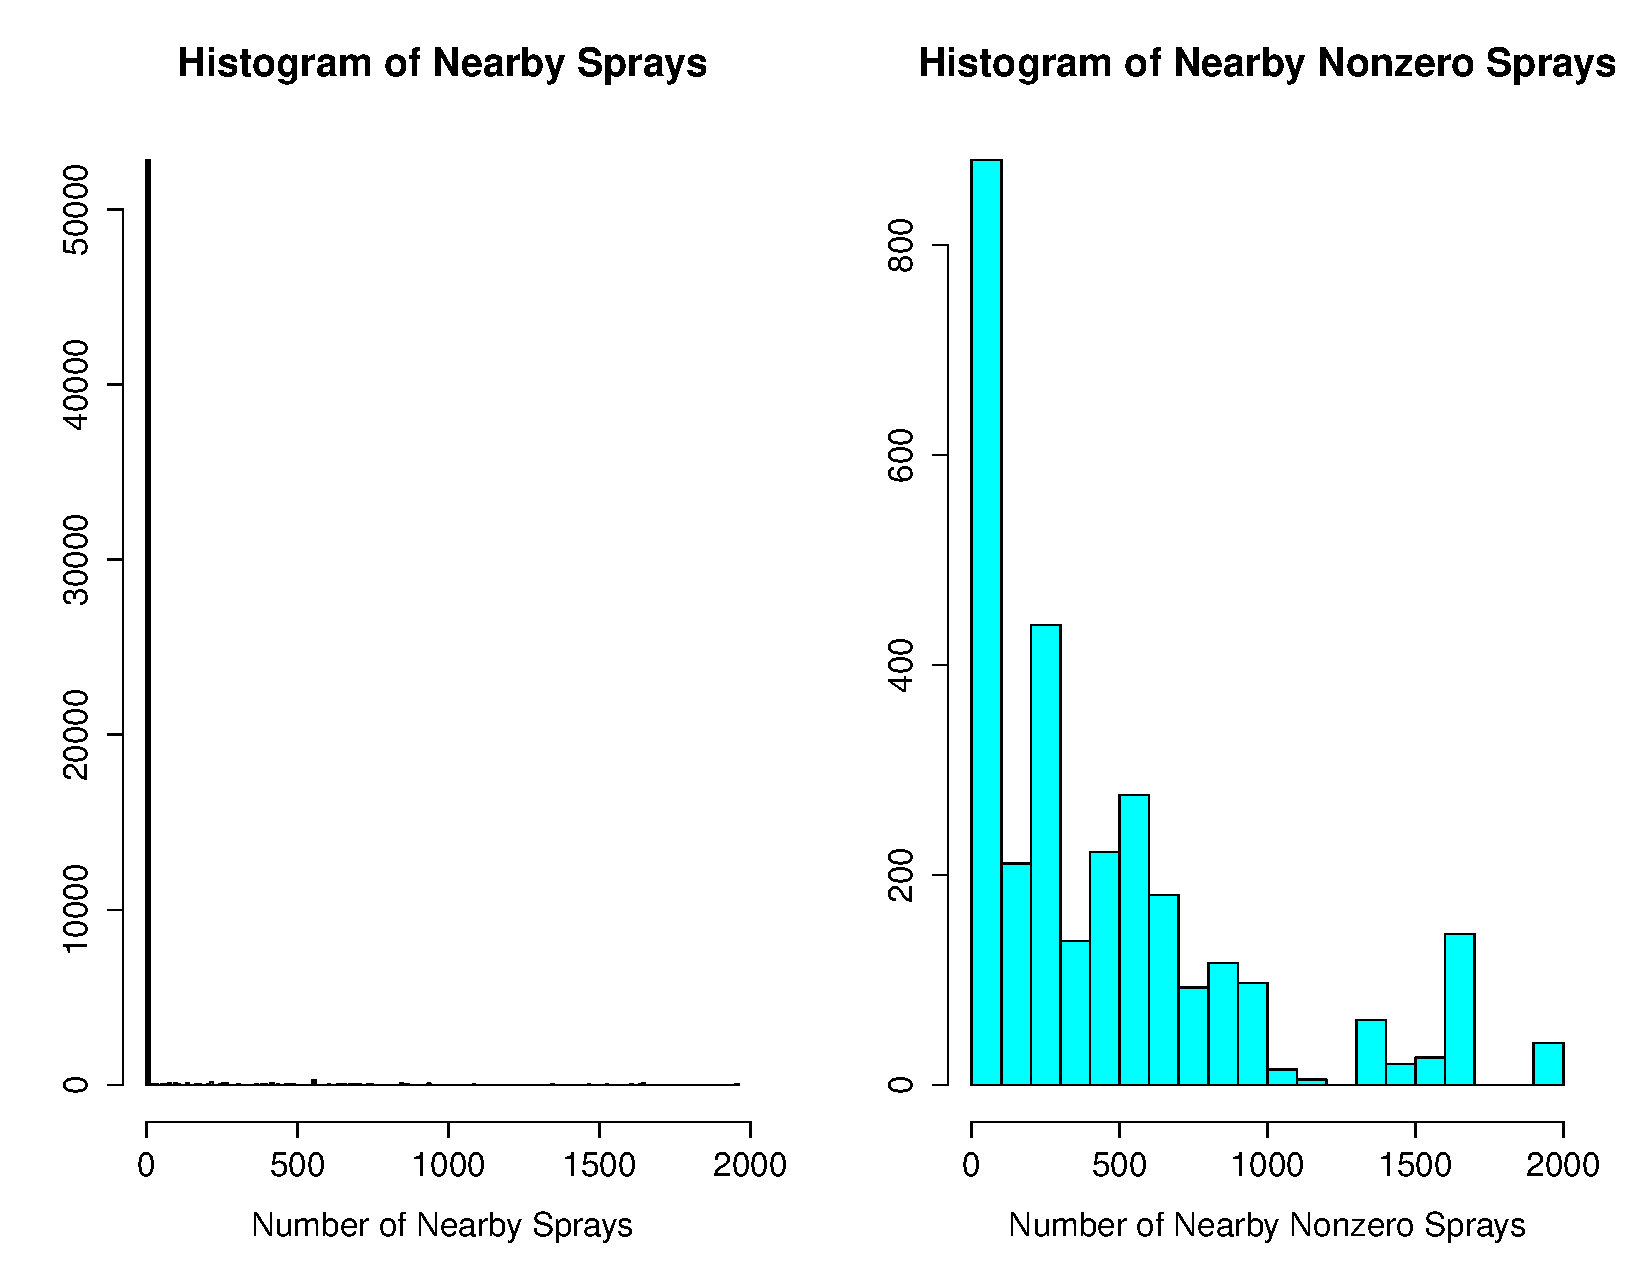
\includegraphics[scale=.60]{Hist_NearbySprays.pdf}
\caption*{Histograms of Number of Nearby Sprays and Number of Non-Zero Sprays}
\end{figure}

\begin{table}[H]
\centering
\begin{tabular}{|c|ccc|} \hline
 & Unpenalized & Unpenalized Boolean & Ridged Dichotomous ($\lambda=3.596$) \\ \hline
Latitude & 1092549.8 & 1089602.8 & 16.2 \\ 
  Longitude & 218429.4 & 217844.1 & 5.6 \\ 
  Tavg & 35.2 & 35.3 & 33.7 \\ 
  DewPoint & 224.5 & 224.5 & 205.0 \\ 
  WetBulb & 324.4 & 325.0 & 296.0 \\ 
  Heat & 3.6 & 3.6 & 3.5 \\ 
  PrecipTotal & 4.9 & 4.9 & 4.8 \\ 
  StnPressure & 179.0 & 179.4 & 168.0 \\ 
  SeaLevel & 184.1 & 184.6 & 172.5 \\ 
  ResultSpeed & 19.2 & 19.2 & 18.8 \\ 
  ResultDir & 1.8 & 1.8 & 1.8 \\ 
  AvgSpeed & 17.7 & 17.9 & 17.6 \\ 
  NearbySprays & 1.0 & 5.2 & 5.0 \\ 
  as.factor(Month)7 & 5.2 & 3.3 & 3.3 \\ 
  as.factor(Month)8 & 3.3 & 3.1 & 3.1 \\ 
  as.factor(Month)9 & 3.1 & 2.4 & 2.4 \\ 
  as.factor(Year)2013 & 2.3 & 1360.9 & 583.0 \\ 
  as.factor(Species)2 & 1360.9 & 2742.7 & 1174.1 \\ 
  as.factor(Species)3 & 2742.7 & 2352.8 & 1007.4 \\ 
  as.factor(Species)4 & 2352.8 & 13.8 & 6.5 \\ 
  as.factor(Species)5 & 13.8 & 2.3 & 1.5 \\ 
  as.factor(Species)6 & 2.3 & 29.0 & 13.0 \\ 
  as.factor(Species)7 & 29.0 & 1.1 & 1.1 \\ 
  Latitude:Longitude & 2046847.0 & 2041333.0 & 27.9 \\ \hline
\end{tabular}
\caption*{Variance Inflation Factors for Logistic Regression with Continuous Spray Count, Dichotomized Spray Count, and Dichotomized Spray Count with Ridge Regression}
\end{table}

\begin{table}[H] \center
\begin{tabular}{|c|cccc|} \hline
 & Estimate & Std. Error & $z$-value & $p$-value \\ 
  \hline
(Intercept) & -41.434 & 450.226 & -0.092 & 0.927 \\ 
  isSpecies1247TRUE & -0.103 & 0.067 & -1.550 & 0.121 \\ 
  Year2013 & -1.052 & 9.158 & -0.115 & 0.909 \\ 
  Month7 & 28.549 & 463.045 & 0.062 & 0.951 \\ 
  Month8 & 38.442 & 464.433 & 0.083 & 0.934 \\ 
  Month9 & 31.644 & 464.695 & 0.068 & 0.946 \\ 
  HeatDegreeDay & 12.919 & 15.203 & 0.850 & 0.395 \\ 
  anyNearbySpraysTRUE & 0.343 & 0.118 & 2.893 & 0.004 \\ 
   \hline
\end{tabular}
\caption*{Output of Linear Terms from GAM on Holdout Data}
\end{table}

\begin{table}[H]
\centering
\begin{tabular}{|r|rrrr|}
  \hline
 & edf & Ref.df & $\chi^2$ & $p$-value \\ 
  \hline
te(Latitude,Longitude) & 23.804 & 23.981 & 345.382 & $\ll 0.0001$ \\ 
  s(Tmax) & 6.058 & 6.150 & 3.061 & 0.815 \\ 
  s(StnPressure) & 5.403 & 5.604 & 2.375 & 0.852 \\ 
  s(ResultSpeed) & 8.179 & 8.190 & 13.190 & 0.114 \\ 
   \hline
\end{tabular}
\caption*{Output of Nonlinear Terms from GAM on Holdout Data}
\end{table}

\begin{figure}[H] \center
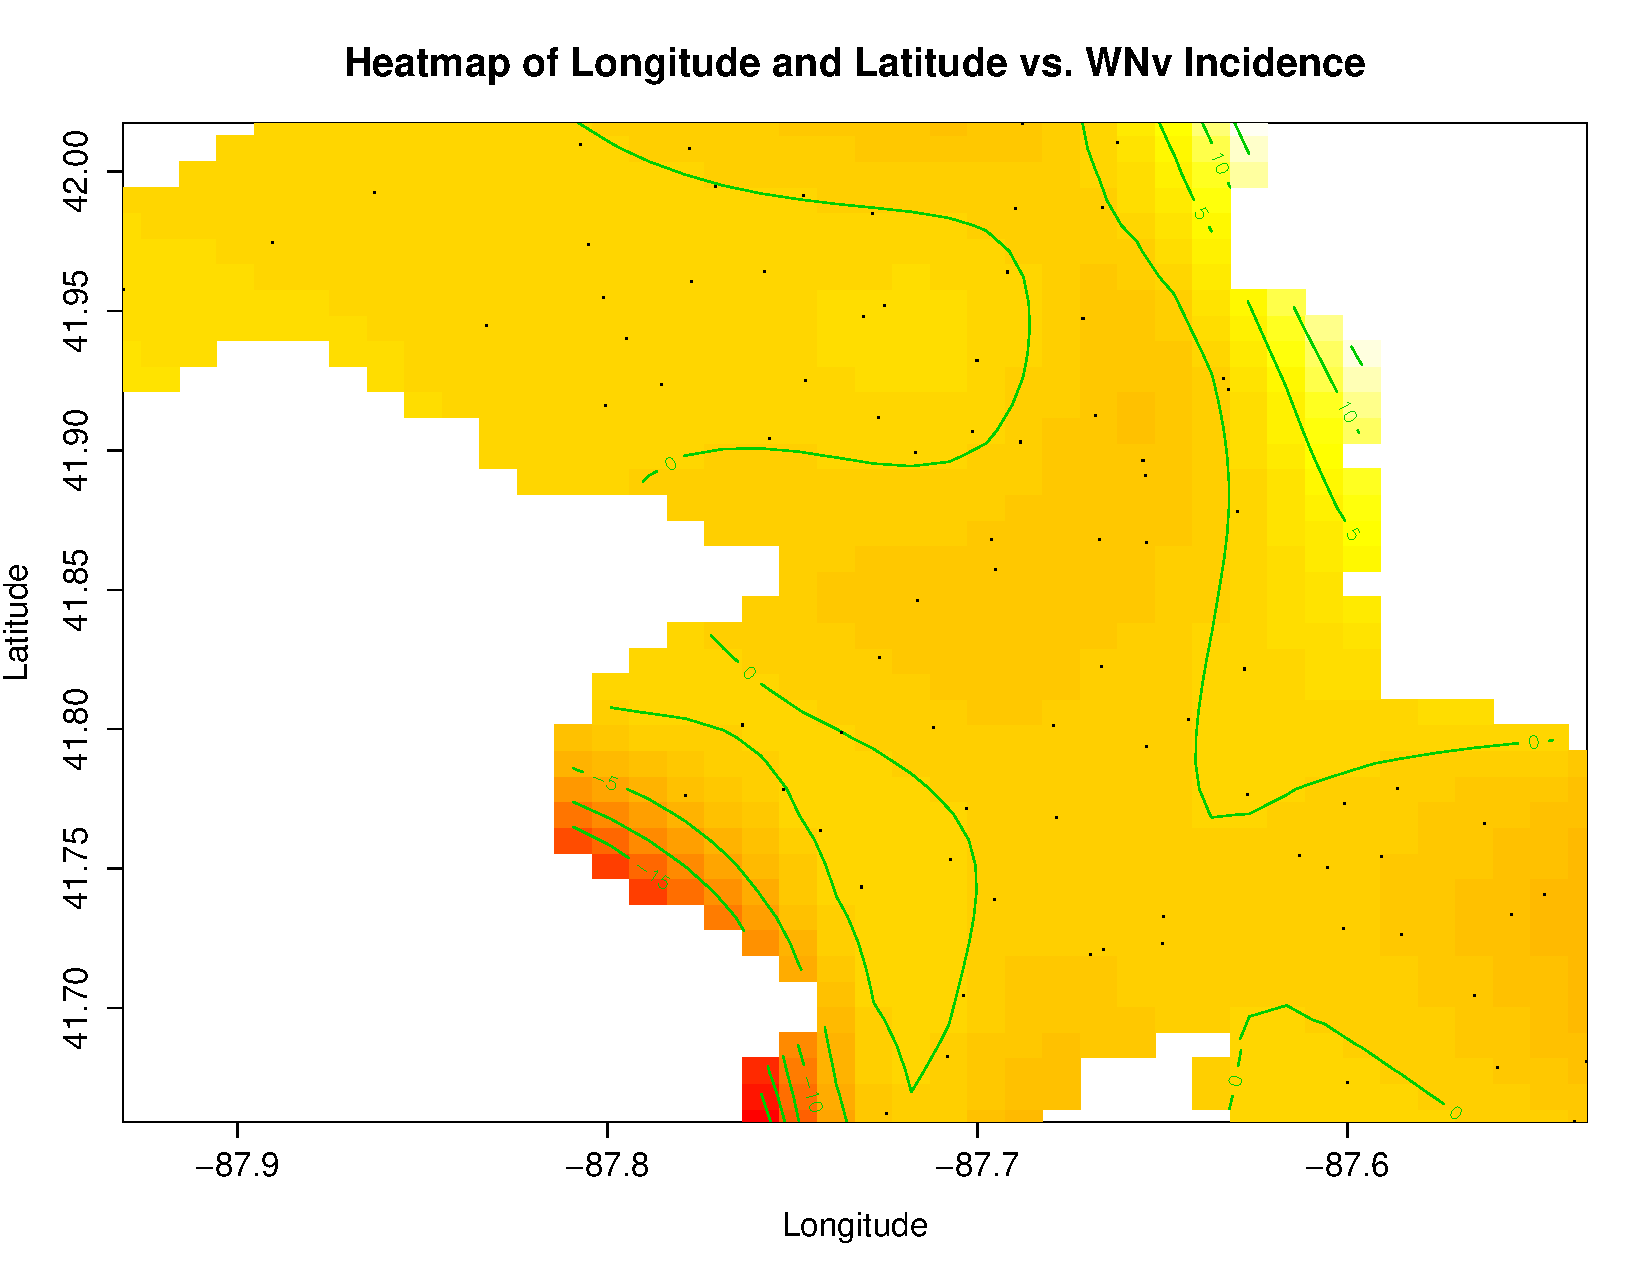
\includegraphics[scale=.60]{LatLongHeat_WNv.pdf}
\caption*{Heatmap of Latitude and Longitude on West Nile Virus incidence}
\end{figure}

\begin{figure}[H] \center
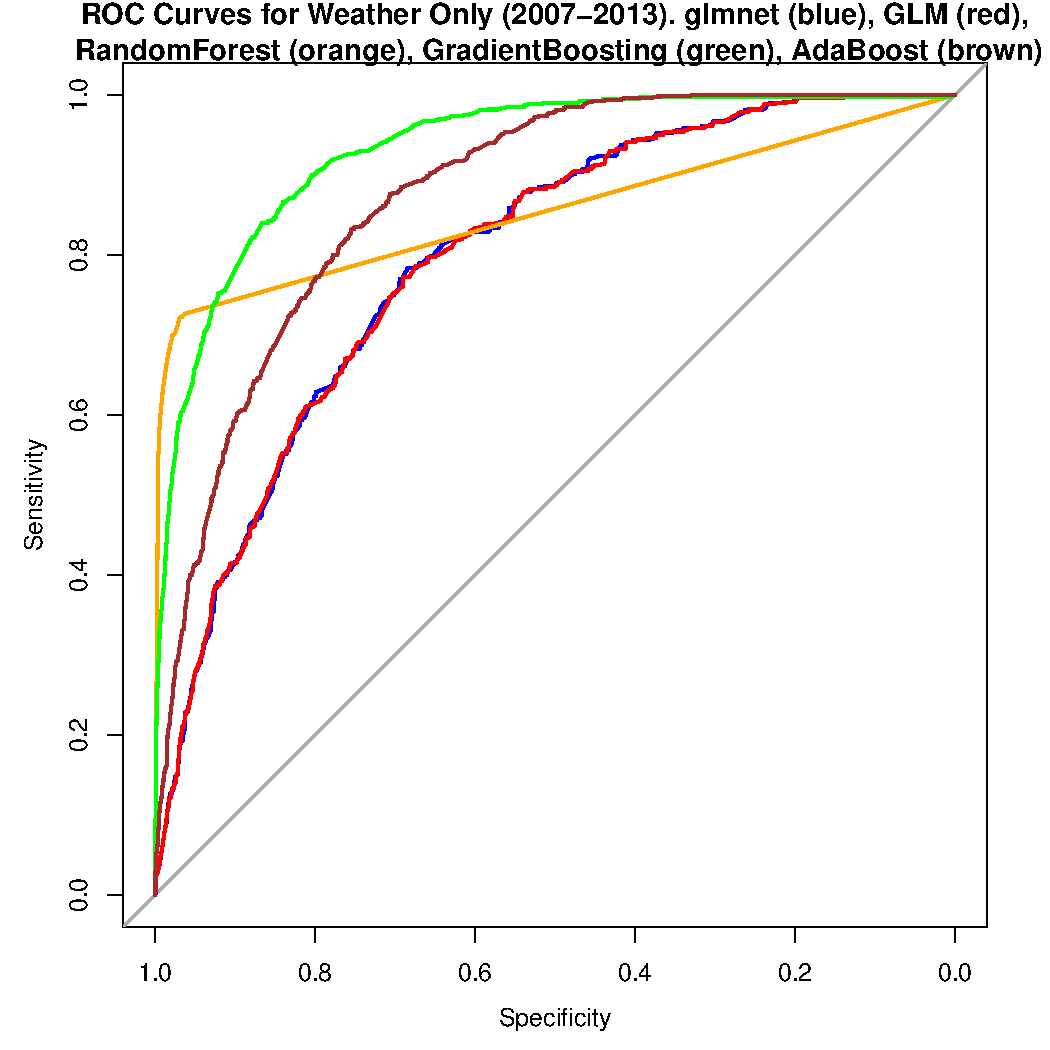
\includegraphics[scale=.50]{ROC_AllYears_Weather.pdf}
\caption*{ROC Curve for All Years Data, Weather \& Trap Predictors}
\end{figure}

\begin{figure}[H] \center
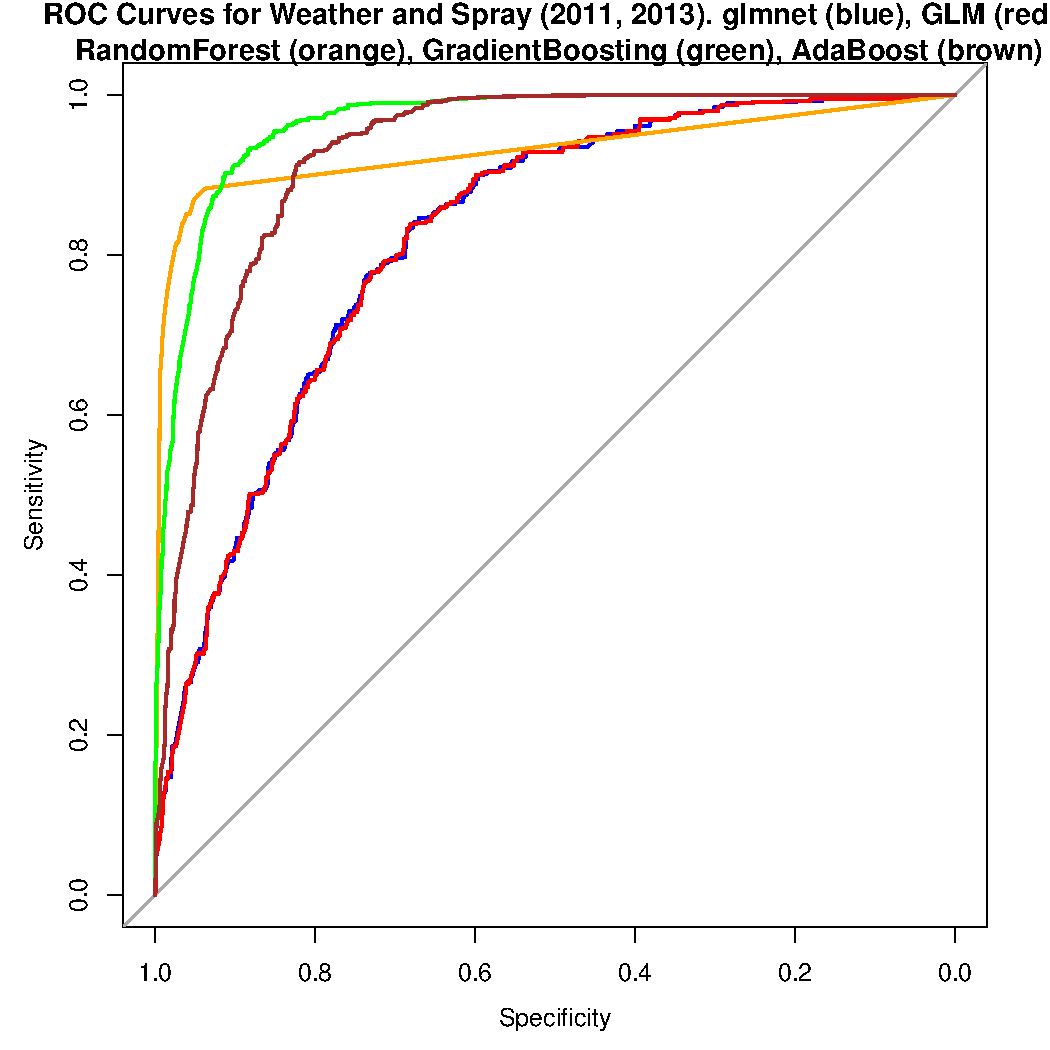
\includegraphics[scale=.50]{ROC_SprayYears_SprayWeather.pdf}
\caption*{ROC Curve for Spray Years, Weather, Trap, \& Spray Predictors}
\end{figure}

\begin{figure}[H] \center
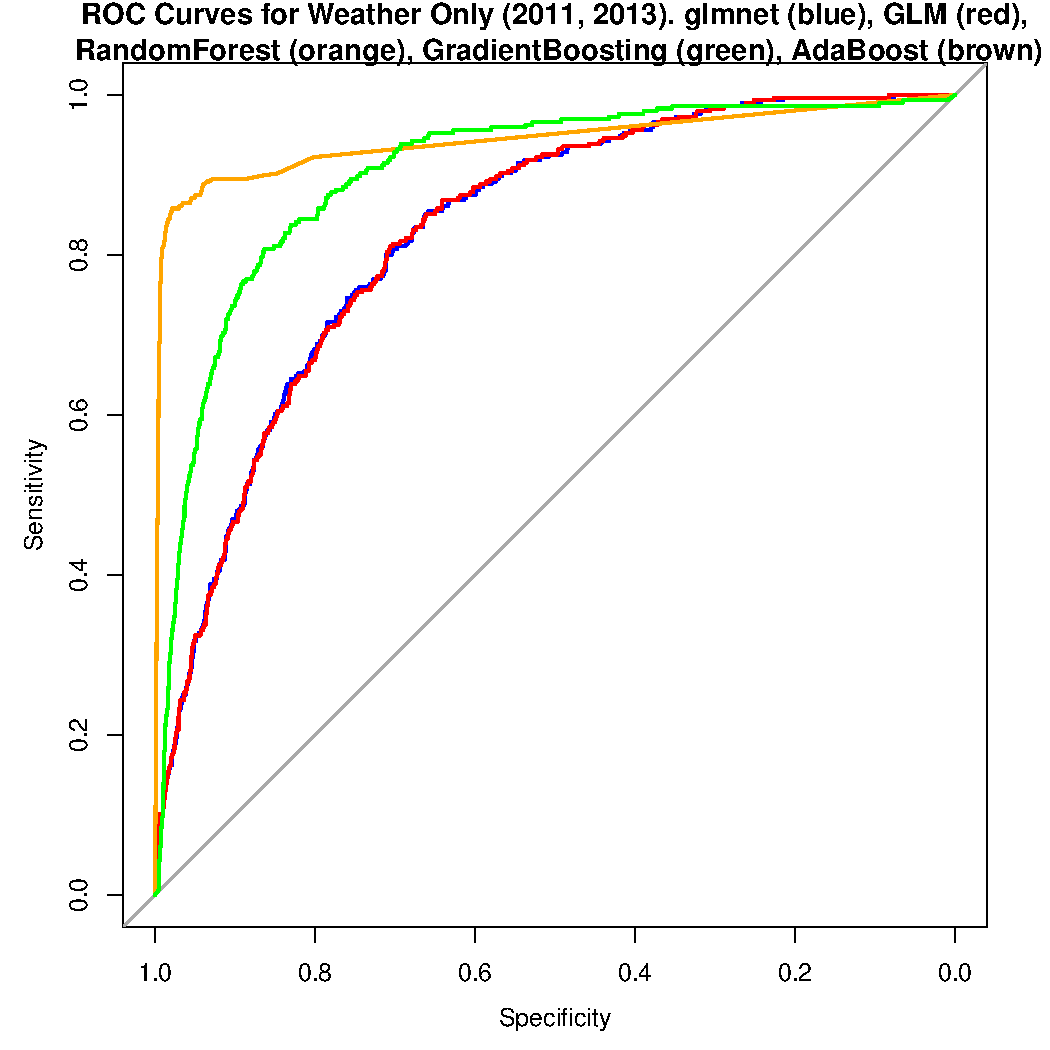
\includegraphics[scale=.60]{ROC_SprayYears_WeatherOnly.pdf}
\caption*{ROC Curve for All Years Data, Weather \& Trap Predictors Only}
\end{figure}

\begin{table}[H] \center \footnotesize
\begin{tabular}{|c|ccc|} \hline
 & Weather AllYears & Weather, SprayYears & Spray \& Weather, SprayYears \\ \hline
GLM & 0.80 & 0.82 & 0.82 \\ 
  GLM Elastic Net & 0.80 & 0.82 & 0.82 \\ 
  RandomForest & 0.85 & 0.93 & 0.93 \\ 
  Gradient Boosting & 0.93 & 0.93 & 0.96 \\ 
  AdaBoost & 0.87 & 0.92 & 0.93 \\ \hline
\end{tabular}
\caption*{Optimal AUCs trained on the whole dataset.}
\end{table}

\newpage
\subsection{Source Code}
All code is available on the personal GitHub repository: \url{https://github.com/christopheraden/BiostatMasters-Oral}. Code is provided here for posterity.

MakeData:
\lstinputlisting{../src/MakeData.R}
Init\_EDA:
\lstinputlisting{../src/Init_EDA.R}
Inference:
\lstinputlisting{../src/Inference.R}
WeatherModel\_Prediction:
\lstinputlisting{../src/WeatherModel_Prediction.R}
Spraying\_Prediction:
\lstinputlisting{../src/Spraying_Prediction.R}
Weather\_Prediction\_Restricted:
\lstinputlisting{../src/Weather_Prediction_Restricted.R}
ROC\_PredictionResults:
\lstinputlisting{../src/ROC_PredictionResults.R}
ConfusionMatrices:
\lstinputlisting{../src/ConfusionMatrices.R}

\newpage
\nocite{*}
\bibliography{Publications}
\bibliographystyle{plain}
\end{document} 